\section{Guidelines}
\begin{figure}[ht]
\centering
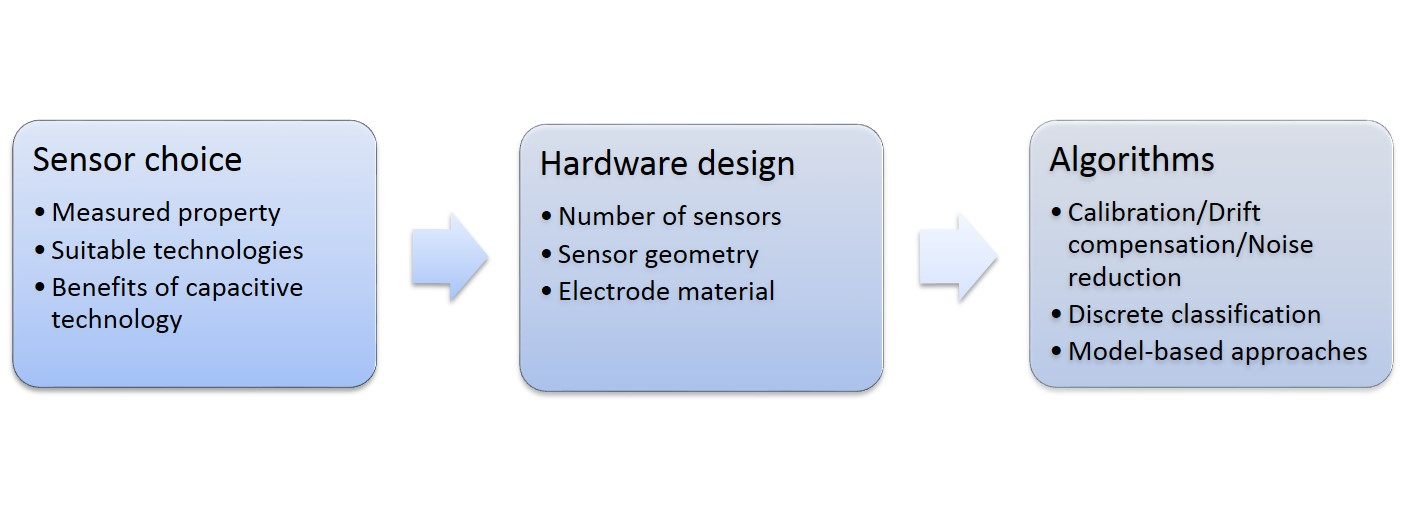
\includegraphics[width=0.8\textwidth]{images/guide_process}
\caption{Basic system design process for capacitive proximity sensing systems and associated aspects in the single steps}
\label{fig:guide_process}
\end{figure}

After discussing the limitations and benefits of capacitive proximity sensors, I am able to use the collected experiences and knowledge to give some general guidelines that can help parties interested in using this sensing technology. These guidelines will support the design process from sensor choice, to choice of algorithms. The process is shown in Figure \ref{fig:guide_process}. This section is structured following the three design steps sensor choice, hardware design, and algorithms. In each subsection a set of questions are posed that are associated to the specific challenges. These questions will be answered with references to the different prototypes created in the scope of this work, and how it influenced the design process.
 
\subsection{Sensor choice}
The first step of this process is the choice of sensor technology for the given application. There is a variety of different options, as presented in Section \ref{ch:sens_compare}. All have their different strengths and weaknesses. In order to decide if capacitive proximity sensing is suitable, three different questions should be posed.

\textit{What do I need to measure in my application scenario?
}

Capacitive proximity sensors can measure the presence and properties of conductive, grounded objects. A prominent object of this category is the human body, having distinct electrical properties. This includes the various application scenarios shown in the previous sections. However, if the application requires measuring properties of unsupported objects that are non-conductive, a different technology should be chosen. In some specific scenarios non-grounded conductive objects can be measured if they are coupled to the electrode. One example is measuring the fluid level of a non-conductive glass container placed on an electrode.

\textit{What sensing technologies are supporting the required measurements?}

It may be the case that multiple technologies support the measurements required in this specific applications. Cameras often can provide similar recognition as capacitive sensors, e.g. in indoor localization applications. In this step all potential sensing technologies should be collected. Additionally, the requirements of the application and constraints towards the environment have to be taken into account. If there are requirements on the visibility of sensing devices, or potential interference due to the unique limitations of a sensor technology, they can be discarded in this step.

\textit{Are capacitive proximity sensors beneficial for my scenario?}

An evaluation of the different candidates is the final step and should lead to a decision about the most suitable sensing technologies. If the distance is too high for capacitive proximity sensors or enough processing power is available and lighting conditions are static, cameras might be more suitable. This should be driven by the different benefits and limitations of the technologies. The benchmarking model presented in Chapter \ref{ch:benchmark} can support this decision process. The designer will have to find the respective feature weights for his applications and calculate the scores for the different sensing systems.

\subsection{Hardware design}
If there has been a decision in favor of capacitive proximity sensors the next step is the design of the hardware.  Similar to technology selection we can use a few basic questions to get an idea of what layout to use.

\textit{How many sensors are required to get the measurement?}

The number of sensors required is depending on the area to be covered, as well as the specific object parameters and the resolution that should be achieved. There is some limitation to the maximum size of the electrodes, as a single sensor can only charge a maximum capacity. However, this theoretical limit is never tested in any of the prototypes presented in this work. If a large area has to be covered more electrodes and sensors are typically used, as the technology is cheap and large electrodes will limit the available resolution. If we just want to measure the presence of a hand a single electrode may suffice. If orientation and position are interesting we need to combine measurements from various sensors. 

We used six electrodes for the MagicBox (\ref{ch:prot_magicbox}) as it is only tracking a single hand on a limited surface. Most prototypes (\ref{ch:prot_smartbed}, \ref{ch:prot_capchair}, \ref{ch:prot_armrest}) use eight sensors as this turned out to be a good compromise providing sufficient data that can be collected by a single sen-sor kit. CapTap (\ref{ch:prot_captap}) uses 24 sensors as we wanted a high resolution over a larger area and CapFloor \ref{ch:prot_capfloor} is scaled to room size and may use a high number of sensors.

\textit{What should be the size and geometry of the electrodes?}

This is closely related to the previous question. If the application is not restricting the available space, the electrode should be approximately of the same size as the object that is to be detected. This generates the highest difference in capacitance when the distance is changing. The Active Armrest (\ref{ch:prot_armrest}) uses six very small electrodes for finger tracking and two larger ones for detecting the arm presence. 

CapFloor (\ref{ch:prot_capfloor}) uses wire electrodes that are spread throughout the room to maximize coverage. The hand tracking devices (\ref{ch:prot_armrest}, \ref{ch:prot_magicbox}) are equipped with hand-sized electrodes and the body sensing devices (\ref{ch:prot_smartbed}, \ref{ch:prot_capchair}) use as much of the available space as possible.

\textit{What is the best electrode material to use?}

Copper is always a good first choice as electrode material. If elasticity is necessary a thin sheet of copper, tin or aluminum can be used. For rigid structure solid PCBs are a good choice, as they also include a copper layer that may be used for shielding. In applications that require transparency, one of the presented materials will have to be used, such as ITO or PEDOT:PSS. Some touch screens also opt for very thin wires that are not visible in typical use with sufficient backlighting. For some applications it is beneficial to integrate electrodes into cloth. In this case there is a variety of conductive threads that may be used. In recent years, printing electronics on paper as become available for home and research applications \cite{kawahara2013instant}. Any conductive material will act as an electrode, thus the application and budget should be the primary driver of this decision. 

Active Armrest and CapTap (\ref{ch:prot_armrest}, \ref{ch:prot_captap}) are not con-strained and use solid copper electrodes. CapFloor (\ref{ch:prot_capfloor}) uses copper wires. MagicBox (\ref{ch:prot_magicbox}) integrates the sensors into a thin casing, thus we used aluminum foil. As we wanted the electrodes of the Smart Bed (\ref{ch:prot_smartbed}) to deform along with the slatted frame we used copper foil. The Capacitive Chair (\ref{ch:prot_capchair}) uses a number of solid copper electrodes but also includes a single conductive thread, as it could be integrated into the mesh structure of the back rest.

\textit{Does my application require any shielding?}

Shielding allows detecting only objects approaching from a certain direction. If the application requires this additional hardware, because it is anticipated that other objects might disturb the measurement, shielding should be used. The only prototype that uses shielding is the CapTap (\ref{ch:prot_captap}), as various electronic devices are integrated into the table and we wanted to minimize disturbance. Shielding however, requires hardware support and comes at additional cost and complexity.

\subsection{Algorithms}
Finally, if the hardware is designed as desired, the different variations of data processing algorithms have to be chosen and configured according to the application.

\textit{What pre-processing algorithms should be used?}

Using baseline calibration is beneficial in the vast majority of applications. Having a distinct starting point simplifies all further steps of high-level data processing, such as normalization and setting different thresholds. This step may only be omitted in very stable environments and if the system has sufficient prior information to operate on raw data. Drift compensation should be handled in a similar fashion. The common methods are not computationally expensive and having a stable baseline over time allows the same algorithms to be applied in a more robust fashion. The method and configuration of noise reduction are strongly depending on the specific case. Some form of noise reduction might be required in most applications. Yet, according to the type of noise different methods can be used. If outliers are an issue a median filter is appropriate; if a smoother signal is desired an average filter can be used. 

In most of the presented prototypes an adaptive baseline calibration is used, together with dynamic normalization, capturing on-the-fly maximum and minimum values. Noise reduction relies mostly on an adaptive average filter that uses a varying sample count based on the extent of changing sensor values, which allows the filtered signal to react more quickly to events.

\textit{What are suitable methods for high-level data processing?}

Regarding high-level data processing there are numerous variations of methods presented in this work. Data-driven machine learning algorithms are a good method, if there is a small set of potential outcomes, e.g. the different postures that could be recognized on a chair or couch. We partially use these methods in the Smart Bed (\ref{ch:prot_smartbed}), on the posture classification of the Capacitive Chair (\ref{ch:prot_capchair}) and for the gesture recognition of the Active Armrest (\ref{ch:prot_armrest}). Of the related prototypes most notably Touché uses these classification methods \cite{Sato2012}. 

If the application has many different potential outcomes, e.g. the thousands of potential locations in a hand tracking system, it is typically beneficial to use a model-driven approach, used in all other prototypes (\ref{ch:prot_capfloor}, localization of Active Armrest\ref{ch:prot_armrest}, \ref{ch:prot_magicbox}, \ref{ch:prot_captap}). However, these models may be supported by data-driven algorithms, such as particle filters. One example is the Swiss-Cheese object tracker by Grosse-Puppendahl et al. \cite{grosse2013swiss}. The data processing examples, shown in Section \ref{ch:prot_proc}, give an idea of the decision rationale in various application domains. 


